% =====================================================================
%  Отчёт по проекту «Экономические убытки сельского хозяйства от засух»
%  Оформление: ГОСТ 7.32-2017 (структура), ГОСТ Р 7.0.5-2008 (ссылки)
%  Компиляция: pdfLaTeX + Biber (рекомендуется Overleaf)
% =====================================================================
\documentclass[14pt,a4paper]{extarticle}

\usepackage[T2A]{fontenc}
\usepackage[utf8]{inputenc}
\usepackage[english,russian]{babel}
\usepackage{tempora}            % Times-подобный шрифт с кириллицей

\usepackage[a4paper,left=30mm,right=15mm,top=20mm,bottom=20mm]{geometry}
\usepackage{setspace}
\onehalfspacing
\setlength{\parindent}{1.25cm}
\emergencystretch=3em   % меньше переполнений строк с длинными \texttt и формулами

\usepackage{amsmath,amssymb}
\usepackage{graphicx}
\graphicspath{{figures/}}
\usepackage{booktabs}
\usepackage{tabularx}
\usepackage{longtable}
\usepackage{array}
\usepackage{float}
\usepackage{caption}
\usepackage{titlesec}
\usepackage{enumitem}
\usepackage{xurl}

% --- подписи по ГОСТ: «Рисунок 1: Название», «Таблица 1, Название» ---
\DeclareCaptionLabelSeparator{gostdash}{~--- }
\captionsetup{labelsep=gostdash, font=normalsize}
\captionsetup[figure]{justification=centering}
\captionsetup[table]{singlelinecheck=false, justification=raggedright}

% --- заголовки разделов: 14 pt полужирные ---
\titleformat{\section}{\normalfont\bfseries\large}{\thesection}{0.6em}{}
\titleformat{\subsection}{\normalfont\bfseries}{\thesubsection}{0.6em}{}
\titlespacing*{\section}{0pt}{12pt}{6pt}
\titlespacing*{\subsection}{0pt}{8pt}{4pt}

% структурные элементы (ВВЕДЕНИЕ, ЗАКЛЮЧЕНИЕ и т.п.), по центру, в оглавление
\newcommand{\structhead}[1]{%
  \clearpage\phantomsection\addcontentsline{toc}{section}{#1}%
  \begin{center}\bfseries\large\MakeUppercase{#1}\end{center}\par\nopagebreak\medskip}

% --- библиография по ГОСТ ---
\usepackage{csquotes}           % требуется biblatex при использовании babel
\usepackage[backend=biber,style=gost-numeric,language=auto,sorting=none]{biblatex}
\addbibresource{references.bib}

\usepackage[hidelinks]{hyperref}

\begin{document}

% =====================================================================
%  ТИТУЛЬНЫЙ ЛИСТ
% =====================================================================
\begin{titlepage}
\centering
{\normalsize
Федеральное государственное автономное образовательное учреждение\\
высшего образования\\
«Национальный исследовательский университет\\
«Высшая школа экономики»\par}
\vfill
{\large\bfseries КУРСОВАЯ РАБОТА\par}
\vspace{6mm}
{\large на тему:\par}
{\Large\bfseries «Экономические убытки сельского хозяйства\\ от негативных природных явлений (засух):\\ оценка на основе индексов засушливости и данных об урожайности»\par}
\vfill
\raggedright
\hspace{60mm}\begin{minipage}{0.5\textwidth}
Выполнил: студент Верпаховский Артём
\end{minipage}
\vfill
\centering
Москва, 2026
\end{titlepage}

% =====================================================================
%  СОДЕРЖАНИЕ
% =====================================================================
\clearpage
\tableofcontents

% =====================================================================
%  ОБОЗНАЧЕНИЯ И СОКРАЩЕНИЯ
% =====================================================================
\structhead{Обозначения и сокращения}
\begin{description}[leftmargin=3.4cm, style=nextline, itemsep=1pt]
\item[АПК] агропромышленный комплекс
\item[НПЯ] негативные (опасные) природные явления
\item[SPI] Standardized Precipitation Index: стандартизированный индекс осадков
\item[SPEI] Standardized Precipitation-Evapotranspiration Index: стандартизированный индекс осадков и испаряемости
\item[PET] потенциальная эвапотранспирация (испаряемость)
\item[ENSO] Эль-Ниньо / Южное колебание
\item[ONI] Oceanic Nino Index: океанический индекс Ниньо
\item[FE] fixed effects: фиксированные эффекты (в панельных моделях)
\item[FAOSTAT] статистическая база данных ФАО ООН
\item[CCKP] Climate Change Knowledge Portal (Всемирный банк)
\item[LOESS] локально взвешенная полиномиальная регрессия (сглаживание)
\end{description}

% =====================================================================
%  ВВЕДЕНИЕ
% =====================================================================
\structhead{Введение}

К негативным природным явлениям (НПЯ) относятся засухи, заморозки, наводнения, лесные пожары и экстремальная жара; все они наносят сельскому хозяйству значительный экономический ущерб. По оценке Продовольственной и сельскохозяйственной организации ООН, на сельское хозяйство приходится непропорционально большая доля потерь от стихийных бедствий, а засухи являются природным явлением, наиболее тяжело сказывающимся на отрасли~\cite{fao2021}. Для России, входящей в число крупнейших производителей и экспортёров зерна, засушливые годы оборачиваются падением сбора зерновых, ростом внутренних цен и угрозами продовольственной безопасности; крупнейшим примером служит катастрофическая засуха и аномальная жара 2010~года~\cite{wegren2011,barriopedro2011}.

\textbf{Актуальность} работы определяется, во-первых, ростом частоты и интенсивности засух в условиях изменения климата~\cite{dai2013}, во-вторых, важностью зернового сектора для экономики и продовольственной безопасности России, и, в-третьих, наличием открытых данных и современных методов, позволяющих количественно оценивать климатические риски АПК.

\textbf{Цель} работы: количественно оценить влияние засух на урожайность зерновых культур и связанные с этим экономические потери на основе реальных открытых данных.

Для достижения цели поставлены следующие \textbf{задачи}:
\begin{enumerate}[leftmargin=*, topsep=2pt, itemsep=1pt]
\item выполнить обзор литературы по экономическим убыткам АПК от НПЯ, индексам засухи и методам оценки связи климата и урожайности;
\item сформировать набор реальных открытых данных (урожайность, климат, цены) и рассчитать индексы засушливости SPI (Standardized Precipitation Index, стандартизированный индекс осадков) и SPEI (Standardized Precipitation-Evapotranspiration Index, стандартизированный индекс осадков и испаряемости);
\item оценить связь засушливости и аномалий урожайности методами корреляционного анализа, панельной регрессии и машинного обучения;
\item оценить денежные потери от недобора урожая в засушливые годы;
\item оформить результаты, программный код и выводы.
\end{enumerate}

\textbf{Объект исследования}: урожайность зерновых культур в России и сопредельных странах зернового пояса; \textbf{предмет}: статистическая связь засушливости с межгодовой изменчивостью урожайности и её экономические последствия.

Работа состоит из четырёх разделов: обзор экономических убытков АПК от НПЯ (раздел~1), постановка задачи (раздел~2), описание и реализация методов (раздел~3), анализ полученных результатов (раздел~4).

% =====================================================================
%  РАЗДЕЛ 1. ОБЗОР
% =====================================================================
\section{Экономические убытки сельского хозяйства от негативных природных явлений}

\subsection{Масштаб потерь АПК и роль засух}

Сельское хозяйство особенно уязвимо к НПЯ, поскольку напрямую зависит от погодных условий. В обзорном докладе ФАО~\cite{fao2021} показано, что на сельское, лесное и рыбное хозяйство приходится значительная доля прямого ущерба от стихийных бедствий в развивающихся странах, причём именно засухи дают наибольшую долю потерь растениеводства и животноводства. C.~Леск с соавторами~\cite{lesk2016} на основе базы стихийных бедствий EM-DAT и данных о национальном производстве зерновых за 1964--2007~гг. методом наложенных эпох показали, что засухи и экстремальная жара снижают национальный сбор зерновых в среднем примерно на $9$--$10\,\%$, тогда как наводнения и ураганы статистически значимого влияния на национальном уровне не оказывают. Авторы также отмечают, что в развитых странах потери от недавних засух выше, чем в развивающихся. Эти работы формируют экономический и методический контекст настоящего исследования.

\subsection{Засухи и индексы засушливости}

Для количественной характеристики засух применяются стандартизированные индексы. Т.~Макки с соавторами~\cite{mckee1993} предложили \emph{стандартизированный индекс осадков} (SPI): накопленные за заданный интервал (1, 3, 6, 12~месяцев) осадки аппроксимируются гамма-распределением и переводятся в стандартную нормальную величину, что позволяет сравнивать засушливость в разных регионах и на разных временны́х масштабах. Недостаток SPI: он учитывает только осадки и не отражает рост испаряемости при потеплении. Этот пробел устранён в \emph{индексе осадков и испаряемости} (SPEI), предложенном С.~Висенте-Серрано с соавторами~\cite{vicenteserrano2010}: SPEI стандартизирует климатический водный баланс (осадки минус потенциальная эвапотранспирация) с помощью трёхпараметрического лог-логистического распределения, сохраняя многомасштабность SPI, но дополнительно реагируя на температурный режим. В развитие метода С.~Бегерия с соавторами~\cite{begueria2014} систематизировали способы оценки параметров распределения и модели расчёта испаряемости (Торнтвейт, Хагривс, Пенман-Монтейт) и опубликовали глобальную базу SPEI и программные средства. Понятие потенциальной эвапотранспирации и температурная формула её расчёта восходят к работе Ч.~Торнтвейта~\cite{thornthwaite1948}, используемой в настоящем проекте. Б.~Ллойд-Хьюз и М.~Сондерс~\cite{lloydhughes2002} построили климатологию засух Европы по индексу SPI за столетний период, продемонстрировав пространственно-временну́ю изменчивость засушливости. А.~Дай~\cite{dai2013} по данным наблюдений и климатических моделей показал тенденцию к усилению засух при глобальном потеплении, что повышает значимость анализа климатических рисков для АПК.

\subsection{Связь климатических экстремумов с урожайностью}

Влияние климата на урожайность исследовано в ряде крупных работ. Д.~Лобелл с соавторами~\cite{lobell2011} с помощью статистических моделей связали тренды температуры и осадков 1980--2008~гг. с мировым производством основных культур и оценили, что потепление снизило глобальные урожаи пшеницы и кукурузы примерно на $5{,}5\,\%$ и $3{,}8\,\%$ относительно сценария без изменения климата. Д.~Рэй с соавторами~\cite{ray2015} показали, что климатическая изменчивость объясняет около трети ($\sim 32$--$39\,\%$) межгодовой изменчивости урожайности кукурузы, риса, пшеницы и сои в мире, а в отдельных «горячих точках», более $60\,\%$. М.~Зампьери с соавторами~\cite{zampieri2017} построили комбинированный индикатор тепловых волн, засухи и переувлажнения и атрибутировали потери урожая пшеницы на глобальном, национальном и субнациональном уровнях, установив доминирующую роль засухи и жары. Т.~Иидзуми с соавторами~\cite{iizumi2014} количественно оценили влияние Эль-Ниньо, Южного колебания (ENSO) на мировые урожаи, показав, что фазы ENSO систематически изменяют урожайность во многих регионах; это обосновывает включение индекса ONI в число объясняющих переменных. На региональном уровне П.~Главинка с соавторами~\cite{hlavinka2009} для Чехии установили тесную связь индексов засухи с детрендированной урожайностью восьми культур, причём наиболее чувствительными оказались яровые культуры. В.~Потопова с соавторами~\cite{potopova2015} показали, что предсказательная сила SPEI зависит от временно́го масштаба и лага, и выделили критические для урожая периоды засушливости.

\subsection{Методы оценки: от корреляций к машинному обучению}

Для моделирования связи климата и урожайности применяют как классические статистические, так и алгоритмические методы. Т.~ван~Кломпенбург с соавторами~\cite{vanklompenburg2020} выполнили систематический обзор более 500~исследований по прогнозированию урожайности методами машинного обучения и показали, что чаще всего используются признаки температуры, осадков и характеристик почвы, а среди алгоритмов преобладают случайный лес и нейронные сети. J.~Чон с соавторами~\cite{jeong2016} продемонстрировали, что случайный лес превосходит множественную линейную регрессию при прогнозировании урожайности на глобальном и региональном уровнях, обеспечивая меньшую ошибку и устойчивость к переобучению. Эти результаты обосновывают выбор градиентного бустинга (CatBoost) и случайного леса в настоящей работе наряду с панельными регрессиями.

\subsection{Засухи и сельское хозяйство России}

Применительно к России климатические риски зернового сектора изучены в нескольких работах. М.~Беляева и Р.~Бокушева~\cite{belyaeva2018} с помощью панельного подхода по регионам России выявили нелинейное влияние температуры на урожайность зерновых, в частности вредоносность экстремально высоких температур; использованный ими панельный анализ с фиксированными эффектами методологически близок к нашему. Ф.~Широхорн с соавторами~\cite{schierhorn2014} количественно оценили разрывы урожайности (yield gaps) в производстве пшеницы в России и показали значительный нереализованный потенциал, особенно в европейской части страны. Н.~Дронин и А.~Кириленко~\cite{dronin2011} рассмотрели историческую связь засух, продовольственного стресса и безопасности в России и подчеркнули уязвимость зернового производства к климатическим экстремумам. С.~Уэгрен~\cite{wegren2011} проанализировал засуху 2010~года: сбор зерна упал примерно с 97 до 61~млн т, был введён запрет на экспорт, выросли цены, с серьёзными последствиями для продовольственной безопасности. Д.~Барриопедро с соавторами~\cite{barriopedro2011} показали, что лето 2010~года переписало температурные рекорды Европы, что объясняет масштаб одновременной засухи и потерь урожая. Контекст динамики посевных площадей в постсоветском пространстве дополнительно раскрыт в работе А.~Прищепова с соавторами~\cite{prishchepov2021}.

\subsection{Сводное сравнение и выводы по обзору}

В таблице~\ref{tab:lit} сопоставлены ключевые рассмотренные работы. Обзор показывает: (1)~засухи: главный источник климатических потерь АПК; (2)~SPEI предпочтительнее SPI в условиях потепления, так как учитывает испаряемость; (3)~климат объясняет существенную, но не доминирующую долю изменчивости урожая; (4)~для России наиболее адекватны панельные и нелинейные (ML) методы. Эти выводы определили постановку задачи и выбор методов настоящей работы.

\begin{table}[H]
\caption{Сводное сравнение ключевых рассмотренных работ}
\label{tab:lit}
\footnotesize
\begin{tabularx}{\textwidth}{>{\raggedright\arraybackslash}p{3.0cm} >{\raggedright\arraybackslash}p{2.6cm} >{\raggedright\arraybackslash}p{3.0cm} >{\raggedright\arraybackslash}X}
\toprule
Источник & Объект / регион & Метод & Ключевой результат \\
\midrule
Макки и др.~\cite{mckee1993} & --- & Гамма-стандартизация осадков & Предложен индекс SPI \\
Висенте-Серрано и др.~\cite{vicenteserrano2010} & Глобально & Лог-логистическая стандартизация $P-\text{PET}$ & Предложен индекс SPEI, чувствительный к потеплению \\
Лобелл и др.~\cite{lobell2011} & Мир, 1980--2008 & Статистические модели & Потепление снизило урожаи пшеницы $\approx 5{,}5\,\%$ \\
Леск и др.~\cite{lesk2016} & 177 стран & Анализ наложенных эпох (EM-DAT) & Засухи снижают сбор зерновых на $\approx 9$--$10\,\%$ \\
Рэй и др.~\cite{ray2015} & Мир & Регрессия по сетке & Климат объясняет $\approx 1/3$ изменчивости урожая \\
Иидзуми и др.~\cite{iizumi2014} & Мир & ENSO vs урожайность & ENSO систематически меняет мировые урожаи \\
Главинка и др.~\cite{hlavinka2009} & Чехия & Корреляции индексов засухи & Яровые культуры наиболее чувствительны \\
Чон и др.~\cite{jeong2016} & Мир/регионы & Случайный лес vs МЛР & RF точнее линейной регрессии \\
Беляева, Бокушева~\cite{belyaeva2018} & Регионы России & Панельная регрессия & Нелинейное влияние температуры на урожай \\
Широхорн и др.~\cite{schierhorn2014} & Россия & Анализ yield gaps & Большой нереализованный потенциал урожайности \\
Уэгрен~\cite{wegren2011} & Россия, 2010 & Кейс-анализ & Сбор зерна упал с~97 до~61 млн т \\
\bottomrule
\end{tabularx}
\end{table}

% =====================================================================
%  РАЗДЕЛ 2. ПОСТАНОВКА ЗАДАЧИ
% =====================================================================
\section{Постановка задачи}

\subsection{Содержательная постановка}

Рассматривается влияние засух на урожайность зерновых культур. \emph{Главный кейс}: Россия; для повышения статистической мощности и робастности в анализ включены сопредельные страны черноморского (постсоветского) зернового пояса со сходными агроклиматическими условиями: Украина, Казахстан, Беларусь, Молдова, Румыния. Требуется: (а)~измерить засушливость количественно (индексы SPI/SPEI и аномалии температуры/осадков вегетационного периода); (б)~оценить статистическую связь засушливости с межгодовой изменчивостью урожайности; (в)~перевести недобор урожая в денежные потери.

\subsection{Формальная постановка}

Пусть $y_{ict}$: урожайность культуры $c$ в стране $i$ в год $t$. Технологический тренд $\hat{y}_{ic}(t)$ (рост за счёт агротехники, сортов, удобрений) оценивается локально взвешенным сглаживанием (LOESS). \emph{Аномалия урожайности} определяется как относительное отклонение от тренда:
\begin{equation}
a_{ict} = \frac{y_{ict} - \hat{y}_{ic}(t)}{\hat{y}_{ic}(t)}\cdot 100\,\%.
\end{equation}
Пусть $D_{it}$: вектор показателей засушливости года $t$ (SPEI разных масштабов, аномалии температуры и осадков лета, индекс ONI). Базовая гипотеза: засушливость снижает урожайность, то есть $\partial a / \partial \text{SPEI} > 0$ и $\partial a / \partial T_{\text{лето}} < 0$. Оцениваются: корреляции $\mathrm{corr}(a, D)$; панельная модель с фиксированными эффектами
\begin{equation}
a_{ict} = \alpha_{ic} + \boldsymbol{\beta}^{\top} D_{it} + \varepsilon_{ict};
\end{equation}
нелинейная модель машинного обучения $a = f(D, \text{страна}, \text{культура}, t) + \varepsilon$. Денежные потери года $t$:
\begin{equation}
L_{t} = \sum_{c} \max\!\big(0,\ \hat{y}_{ct}-y_{ct}\big)\cdot A_{ct}\cdot p_{ct},
\end{equation}
где $A_{ct}$: убранная площадь, $p_{ct}$: цена производителя.

\subsection{Уровень сложности и план усложнения}

Работа выстроена по возрастанию сложности: от корреляций (базовый уровень) к панельным регрессиям с фиксированными эффектами и далее к моделям машинного обучения с денежной оценкой убытков. \textbf{План дальнейшего усложнения:} (1)~переход на субнациональный уровень (урожайность по регионам/областям и климат по зернопроизводящим районам, это устранит «разбавление» сигнала при усреднении по всей территории страны); (2)~учёт фенологических фаз и культуроспецифичных вегетационных окон; (3)~добавление данных дистанционного зондирования (NDVI, влажность почвы); (4)~имитационное моделирование роста культур (например, AquaCrop) и сценарии изменения климата; (5)~эконометрическое выделение эффекта засух на цены и экспорт.

\subsection{Данные}

Использованы только реальные открытые данные (даты выгрузки и ссылки, в \texttt{data/README.md} репозитория): урожайность, площади и валовой сбор, а также цены производителей, FAOSTAT~\cite{faostat2026}; месячные осадки и температура (CRU~TS~4.07), Climate Change Knowledge Portal Всемирного банка~\cite{cckp2026}; индекс ENSO (ONI): NOAA~\cite{noaaoni2026}. Корректность чтения FAOSTAT дополнительно сверена с рядами World Bank Open Data и Our World in Data; оба ряда производны от данных ФАО, поэтому служат контролем согласованности, а не независимой валидацией (последняя потребовала бы национальной статистики, например Росстата). Для уточнения пространственного масштаба использованы сеточные данные NOAA PSL: осадки GPCC~\cite{gpcc2013} и температура GHCN-CAMS~\cite{ghcncams2008}.

% =====================================================================
%  РАЗДЕЛ 3. МЕТОДЫ И РЕАЛИЗАЦИЯ
% =====================================================================
\section{Выбранные методы оценки и их реализация}

\subsection{Расчёт индексов засухи}

Потенциальная эвапотранспирация рассчитана по методу Торнтвейта~\cite{thornthwaite1948} с поправкой на продолжительность светового дня по широте зернопроизводящих районов каждой страны. Индекс SPI получен стандартизацией накопленных за $k$~месяцев осадков через гамма-распределение~\cite{mckee1993}; индекс SPEI: стандартизацией накопленного климатического водного баланса $D=P-\text{PET}$ через трёхпараметрическое лог-логистическое распределение методом взвешенных моментов~\cite{vicenteserrano2010,begueria2014}. Распределения калибровались отдельно для каждого календарного месяца по периоду 1901--2022~гг. Рассчитаны SPI и SPEI масштабов 3, 6 и 12~месяцев; для анализа использованы значения на конец вегетационного периода (август). Реализация: в модуле \texttt{src/spei.py} без использования внешних пакетов индексов засухи, что обеспечивает прозрачность расчёта (\emph{собственная реализация методов}).

\subsection{Аномалии урожайности и признаки}

Технологический тренд урожайности оценён сглаживанием LOESS (доля $0{,}5$); аномалия вычислена по формуле~(1). Климатические признаки года: SPEI-3/6/12 и SPI-6 на конец вегетации, годовой SPEI-12, стандартизованные аномалии температуры и осадков лета (май--август), индекс ONI за зиму, весну и лето. Сборка панели «страна\,$\times$\,год\,$\times$\,культура» реализована в \texttt{src/01\_build\_panel.py}.

\subsection{Корреляционный анализ}

Рассчитаны коэффициенты корреляции Пирсона и Спирмена между аномалиями урожайности и показателями засушливости, по отдельным странам и в объединённой панели с предварительным вычитанием страновых средних (аналог фиксированных эффектов).

\subsection{Панельные регрессии с фиксированными эффектами}

Оценены три спецификации модели~(2) с помощью \texttt{linearmodels.PanelOLS} со стандартными ошибками Дрисколла–Краая (устойчивы к зависимости между странами): (A)~пшеница, фиксированные эффекты стран; (B)~все культуры, фиксированные эффекты «страна\,$\times$\,культура»; (C)~пшеница, фиксированные эффекты стран и годов (контроль общих для всех стран шоков). Реализация: \texttt{src/03\_panel\_regression.py}.

\subsection{Машинное обучение}

Аномалия урожайности моделировалась тремя методами: линейная регрессия (база), случайный лес и градиентный бустинг CatBoost. Использованы только климатические признаки (включая лаг засушливости предыдущего года, пиковую жару лета и внутрисезонный минимум SPEI). Обобщающая способность оценивалась двумя схемами кросс-валидации: \emph{стандартной} повторной случайной ($5\times5$ блоков; сопоставимо с обзором~\cite{vanklompenburg2020}) и \emph{строгой} групповой по годам (\texttt{GroupKFold}: прогноз для целиком не входивших в обучение лет). Оценивались $R^2$, RMSE и MAE; для CatBoost построены важности признаков и частные зависимости. Реализация: \texttt{src/04\_ml\_model.py}.

\subsection{Оценка денежных убытков}

Недобор урожая в год $t$ относительно технологического тренда переводился в физические потери (т) умножением на убранную площадь и далее в денежные (долл. США) умножением на цену производителя соответствующей культуры FAOSTAT по формуле~(3). Суммирование велось по зерновым (пшеница, ячмень, кукуруза, овёс, рожь). Реализация: \texttt{src/05\_economic\_loss.py}.

\subsection{Программная реализация}

Весь пайплайн написан на Python (numpy, pandas, scipy, statsmodels, linearmodels, scikit-learn, CatBoost, matplotlib) и полностью воспроизводим: команда \texttt{python src/run\_all.py} выполняет загрузку данных и все этапы анализа. Структура репозитория приведена в приложении~А.

% =====================================================================
%  РАЗДЕЛ 4. АНАЛИЗ РЕЗУЛЬТАТОВ
% =====================================================================
\section{Анализ проделанной работы и полученных результатов}

\subsection{Разведочный анализ}

На рис.~\ref{fig:trend} показана урожайность пшеницы в России и технологический тренд: на фоне устойчивого роста (с $\approx 1{,}5$ до $\approx 3{,}1$~т/га) отчётливо видны провалы в засушливые 2010 и 2012~годы. Рисунок~\ref{fig:speits} представляет динамику индекса SPEI-6: засухи 2010, 2012 и 2021~годов выделяются значениями ниже порога $-1$.

\begin{figure}[H]
\centering
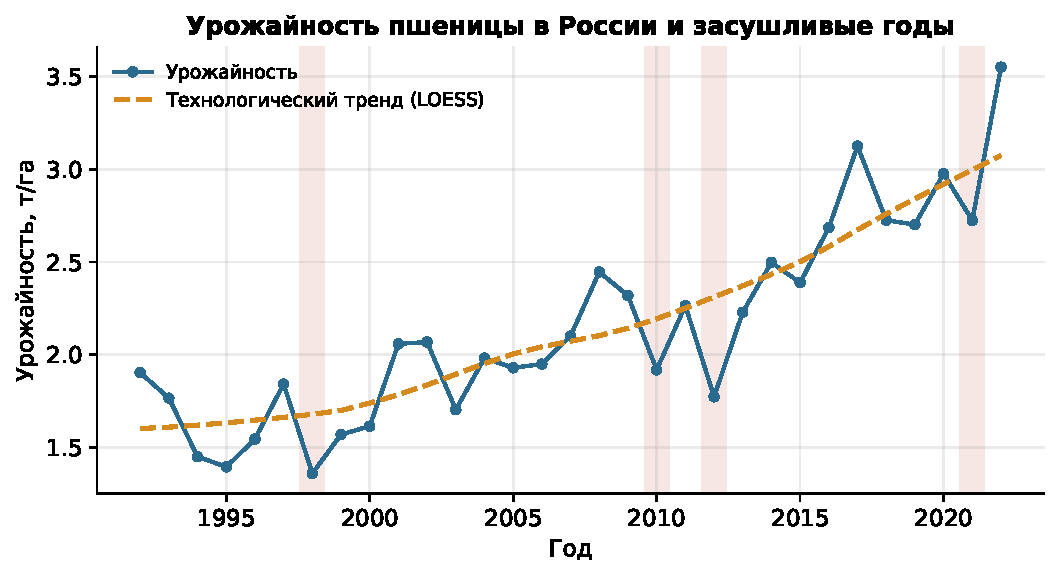
\includegraphics[width=0.85\textwidth]{fig01_russia_yield_trend.pdf}
\caption{Урожайность пшеницы в России и технологический тренд (LOESS); засушливые годы выделены. Источник: составлено авторами по данным FAOSTAT~\cite{faostat2026}}
\label{fig:trend}
\end{figure}

\begin{figure}[H]
\centering
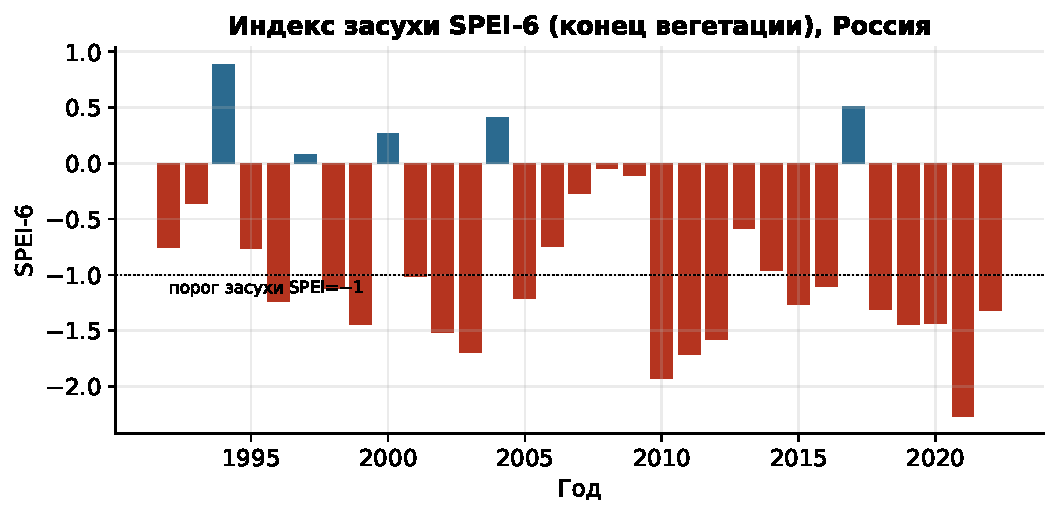
\includegraphics[width=0.85\textwidth]{fig04_russia_spei_timeseries.pdf}
\caption{Индекс засухи SPEI-6 (конец вегетации) для России. Источник: расчёты авторов по данным CCKP~\cite{cckp2026}}
\label{fig:speits}
\end{figure}

\subsection{Корреляционный анализ}

Для России связь аномалии урожайности пшеницы с SPEI положительна и значима на длинных масштабах (SPEI-12: $r=0{,}36$, $p=0{,}05$; SPEI-6: $r=0{,}32$, $p=0{,}08$; рис.~\ref{fig:scatter}). Простой индекс осадков SPI на национальном уровне сигнал почти не улавливает, что подтверждает важность учёта испаряемости (температуры), то есть преимущество SPEI над SPI в условиях, когда засуха связана с жарой. В объединённой панели с фиксированными эффектами стран связь существенно сильнее: для SPEI-6 $r=0{,}42$, для аномалии температуры лета $r=0{,}38$ (оба $p<0{,}001$). По странам (рис.~\ref{fig:bars}) сигнал максимален в степных Казахстане и Молдове и минимален во влажной Беларуси, что физически закономерно.

\begin{figure}[H]
\centering
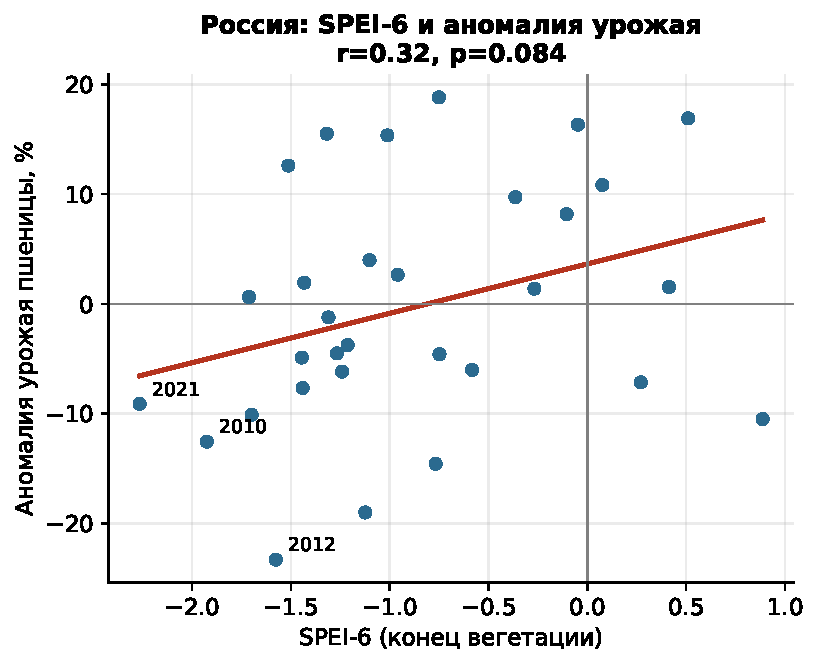
\includegraphics[width=0.62\textwidth]{fig02_russia_spei_yield_scatter.pdf}
\caption{Связь SPEI-6 и аномалии урожая пшеницы, Россия. Источник: расчёты авторов по данным FAOSTAT~\cite{faostat2026} и CCKP~\cite{cckp2026}}
\label{fig:scatter}
\end{figure}

\begin{figure}[H]
\centering
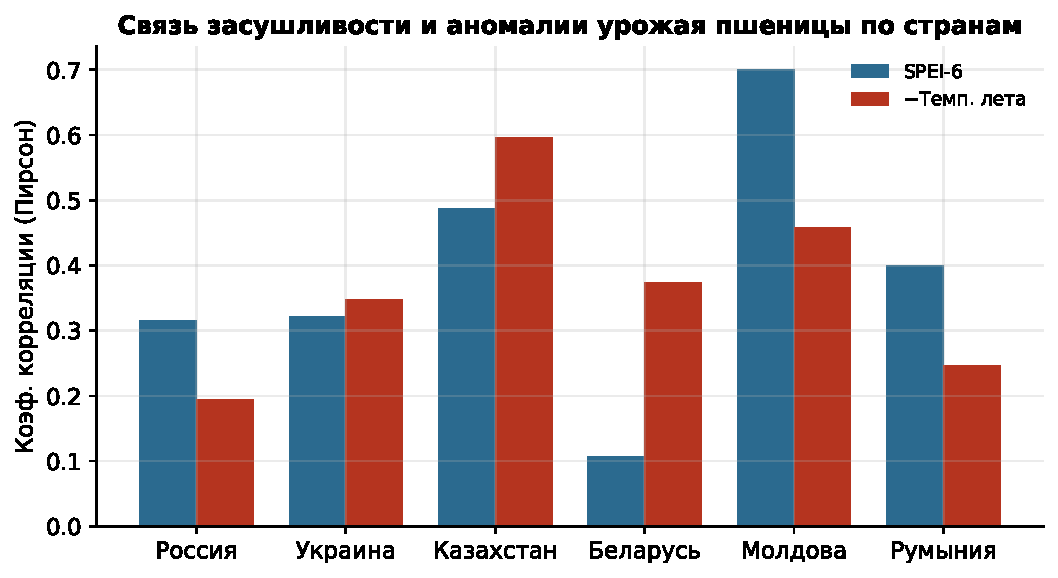
\includegraphics[width=0.85\textwidth]{fig03_country_corr_bars.pdf}
\caption{Корреляция засушливости и аномалии урожая пшеницы по странам. Источник: расчёты авторов}
\label{fig:bars}
\end{figure}

\subsection{Панельные регрессии}

Результаты панельных моделей приведены в таблице~\ref{tab:panel}. Точечные оценки во всех спецификациях показывают положительную связь SPEI-6 с урожаем: повышение SPEI на одно стандартное отклонение соответствует приросту урожайности на $4$--$6\,\%$. Связь статистически значима в моделях~(A) и~(B) ($p<0{,}01$). В наиболее строгой модели~(C) с фиксированными эффектами и стран, и годов эффект SPEI ослабевает и теряет значимость ($p\approx0{,}15$), тогда как определяющим становится отрицательный эффект жары лета ($-7{,}5\,\%$ на стандартное отклонение, $p<0{,}10$). Это содержательный результат: засухи в соседних странах во многом синхронны, поэтому годовые фиксированные эффекты поглощают их общую компоненту, оставляя внутри года прежде всего температурный стресс. Стандартные ошибки рассчитаны по методу Дрисколла–Краая, устойчивому к гетероскедастичности, автокорреляции и межстрановой зависимости (важной из-за общих глобальных шоков). Объяснённая внутригрупповая доля дисперсии ($R^2_{\text{внутр.}}$) достигает $0{,}21$.

\begin{table}[H]
\caption{Панельные регрессии аномалии урожайности (зависимая переменная: аномалия урожая, \%)}
\label{tab:panel}
\centering
\begin{tabular}{lccc}
\toprule
 & (A) Пшеница & (B) Все культуры & (C) Пшеница \\
 & FE стран & FE страна$\times$культура & FE стран+годов \\
\midrule
SPEI-6 (вегетация) & 5.49$^{***}$ (1.91) & 5.71$^{***}$ (1.28) & 4.27 (2.93) \\
Темп. лета (z) & -2.32 (2.92) & -0.47 (2.35) & -7.46$^{*}$ (4.40) \\
ONI (лето) & 3.64$^{**}$ (1.67) & 2.57 (1.68) & -- \\
\midrule
Набл. & 186 & 1488 & 186 \\
$R^2$ (внутр.) & 0.21 & 0.12 & 0.14 \\
\bottomrule
\end{tabular}

\smallskip
\footnotesize В скобках: стандартные ошибки Дрисколла–Краая. $^{*}$, $^{**}$, $^{***}$: значимость на уровне $10$, $5$, $1\,\%$. Источник: расчёты авторов.
\end{table}

\subsection{Машинное обучение и важность факторов}

При стандартной (случайной повторной) кросс-валидации модели CatBoost и случайного леса объясняют около $37\,\%$ дисперсии аномалий урожая ($R^2=0{,}37$), заметно превосходя линейную регрессию ($R^2=0{,}19$); это согласуется с мировыми оценками вклада климата в изменчивость урожая~\cite{ray2015}. Однако при строгой проверке на целиком не входивших в обучение годах качество падает до $R^2\approx0{,}07$: предсказать исход конкретного нового года по \emph{усреднённому по стране} климату трудно. Сам разрыв между двумя оценками показателен: значительная часть объяснительной силы приходится на пространственную синхронность засух (наблюдения соседних стран того же года), а не на способность прогнозировать новый год. В числе важнейших признаков (рис.~\ref{fig:imp}) преобладают индексы засушливости и температурные переменные. Частные зависимости (рис.~\ref{fig:pdp}) физически согласованы: урожайность растёт с ростом SPEI и резко падает при экстремальной жаре лета. Вывод: климат вносит реальный, но не доминирующий вклад; бо́льшая часть изменчивости урожая обусловлена неклиматическими факторами (агротехника, экономика, политика).

\begin{figure}[H]
\centering
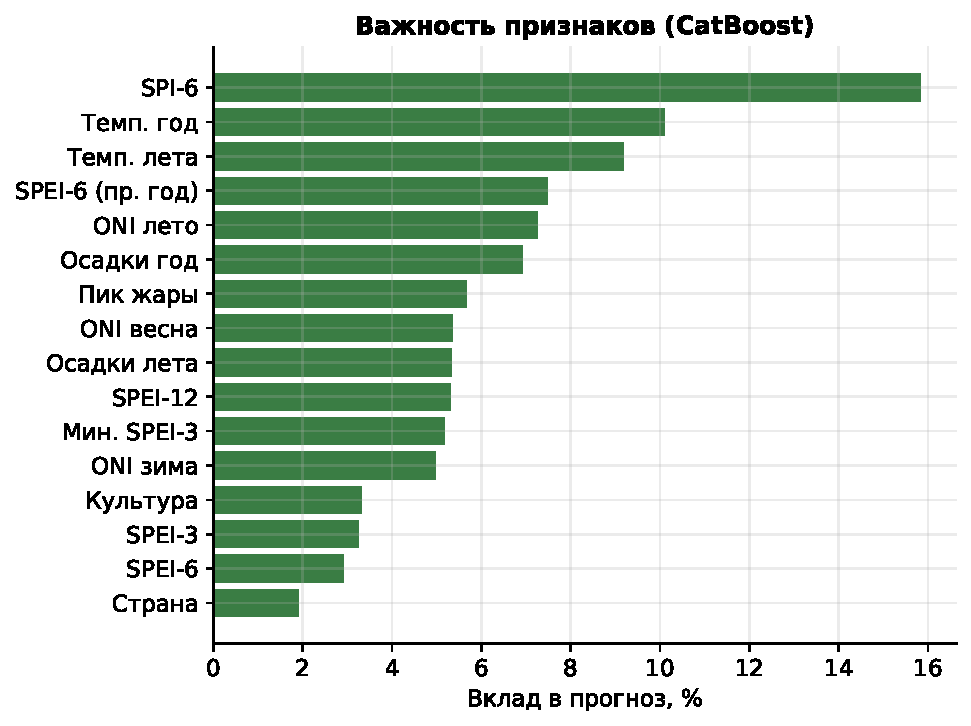
\includegraphics[width=0.72\textwidth]{fig05_feature_importance.pdf}
\caption{Важность признаков в модели CatBoost. Источник: расчёты авторов}
\label{fig:imp}
\end{figure}

\begin{figure}[H]
\centering
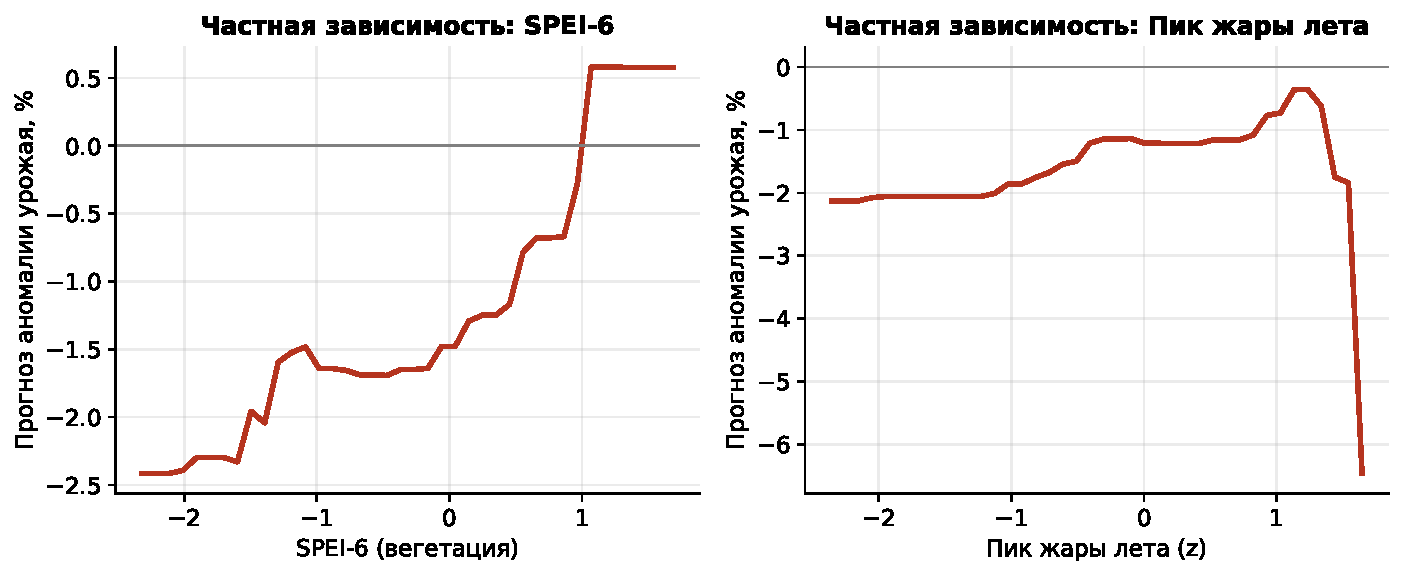
\includegraphics[width=0.95\textwidth]{fig06_partial_dependence.pdf}
\caption{Частные зависимости прогноза аномалии урожая от SPEI-6 и температуры лета. Источник: расчёты авторов}
\label{fig:pdp}
\end{figure}

\begin{figure}[H]
\centering
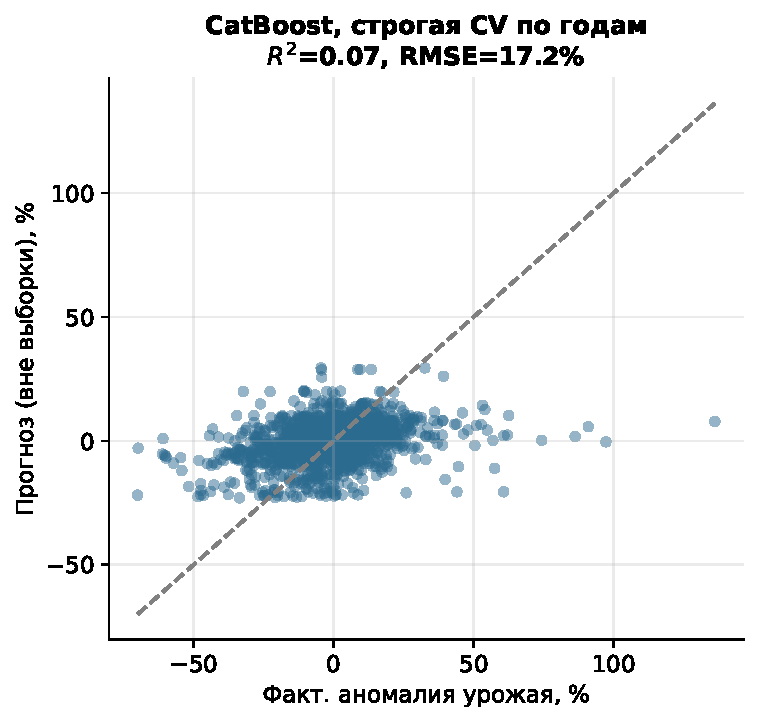
\includegraphics[width=0.55\textwidth]{fig07_pred_vs_actual.pdf}
\caption{Прогноз CatBoost вне обучающей выборки против факта. Источник: расчёты авторов}
\label{fig:pva}
\end{figure}

\subsection{Экономические убытки}

Оценка прямых потерь сбора зерновых России (рис.~\ref{fig:loss}) выделяет засушливые годы: 2012, 2010, 2021 и 1995. По базовому контрфакту (тренд LOESS, текущие цены) недобор 2012~года составляет $\approx14{,}7$~млн т ($\approx3{,}0$~млрд долл. США, или $18\,\%$ ожидаемой стоимости продукции); для 2010~года потери равны $\approx9{,}8$~млн т ($\approx1{,}2$~млрд долл.), для 2021~года $\approx2{,}0$~млрд долл. Для проверки робастности убытки пересчитаны при втором контрфакте (среднее за три предыдущих года) и в постоянных ценах 2014--2020~гг.: оценки отдельных засушливых лет лежат в диапазоне $1$--$3$~млрд долл., а накопленные потери за 2000--2022~гг., от $6{,}5$ до $11$~млрд долл. Для 2010~года при базе «среднее за три года» оценка возрастает до $\approx1{,}6$--$1{,}8$~млрд долл.; занижение в базовом варианте объясняется низкой ценой производителя 2010~года и свойством LOESS частично «впитывать» кластеры засушливых лет. Косвенные макроэкономические потери (запрет экспорта, удорожание кормов, эффекты на смежные отрасли) в оценку не входят и в литературе для 2010~года существенно выше~\cite{wegren2011}.

\begin{figure}[H]
\centering
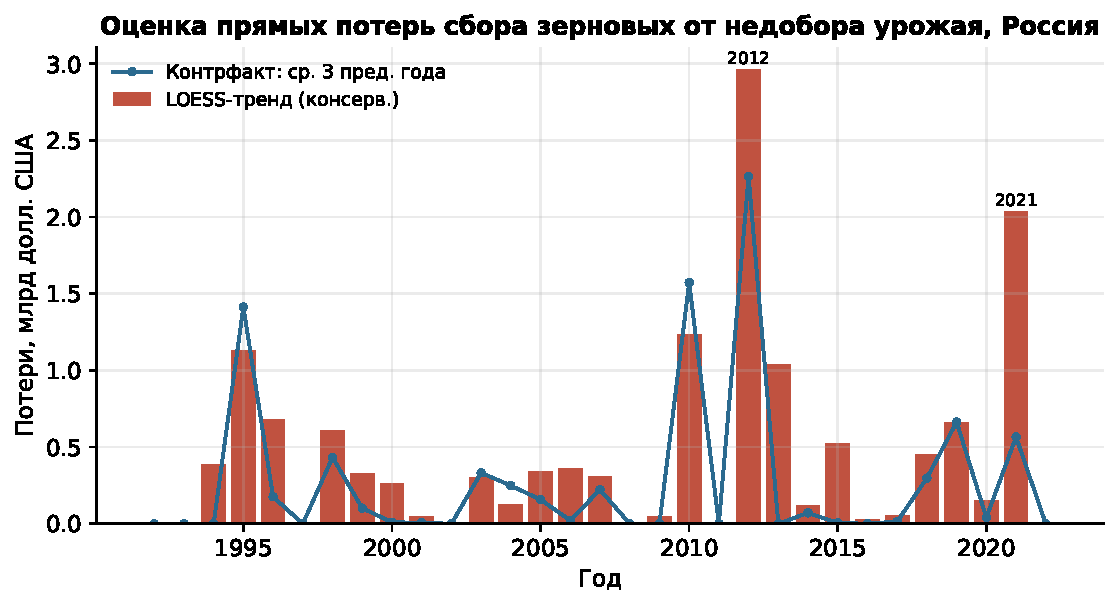
\includegraphics[width=0.85\textwidth]{fig08_economic_loss.pdf}
\caption{Оценка прямых потерь сбора зерновых от недобора урожая, Россия. Источник: расчёты авторов по данным FAOSTAT~\cite{faostat2026}}
\label{fig:loss}
\end{figure}

\subsection{Уточнение пространственного масштаба: климат зернового пояса}

Главное ограничение национального анализа: усреднение климата по всей территории страны, размывающее сигнал. Чтобы проверить и снять его, климат пересчитан только по \emph{зернопроизводящему поясу} (европейская Россия, Поволжье, Южный Урал; бокс $45$--$56^{\circ}$\,с.\,ш., $38$--$62^{\circ}$\,в.\,д.) по сеточным данным: осадки GPCC~\cite{gpcc2013} и температура GHCN-CAMS~\cite{ghcncams2008} (NOAA PSL~\cite{noaapsl2026}). Результат (рис.~\ref{fig:belt}) подтверждает гипотезу: связь аномалии урожая с засушливостью пояса заметно сильнее национальной (сравнение за общий период 1992--2019, поэтому национальный коэффициент здесь немного отличается от раздела~4.2). Корреляция аномалии урожая с SPEI-6 возрастает с $0{,}34$ до $0{,}43$, а с аномалией летней температуры растёт с $0{,}26$ (незначимо) до $0{,}48$ ($p=0{,}01$). Индекс SPEI пояса для засухи 2010~года достигает $-2{,}55$ против $-1{,}93$ по стране, поэтому экстремальная засуха европейской части России перестаёт «теряться» в национальном среднем. Тем самым основное ограничение во многом снимается уже на стороне климата; следующий шаг: субнациональные данные \emph{урожайности}.

\begin{figure}[H]
\centering
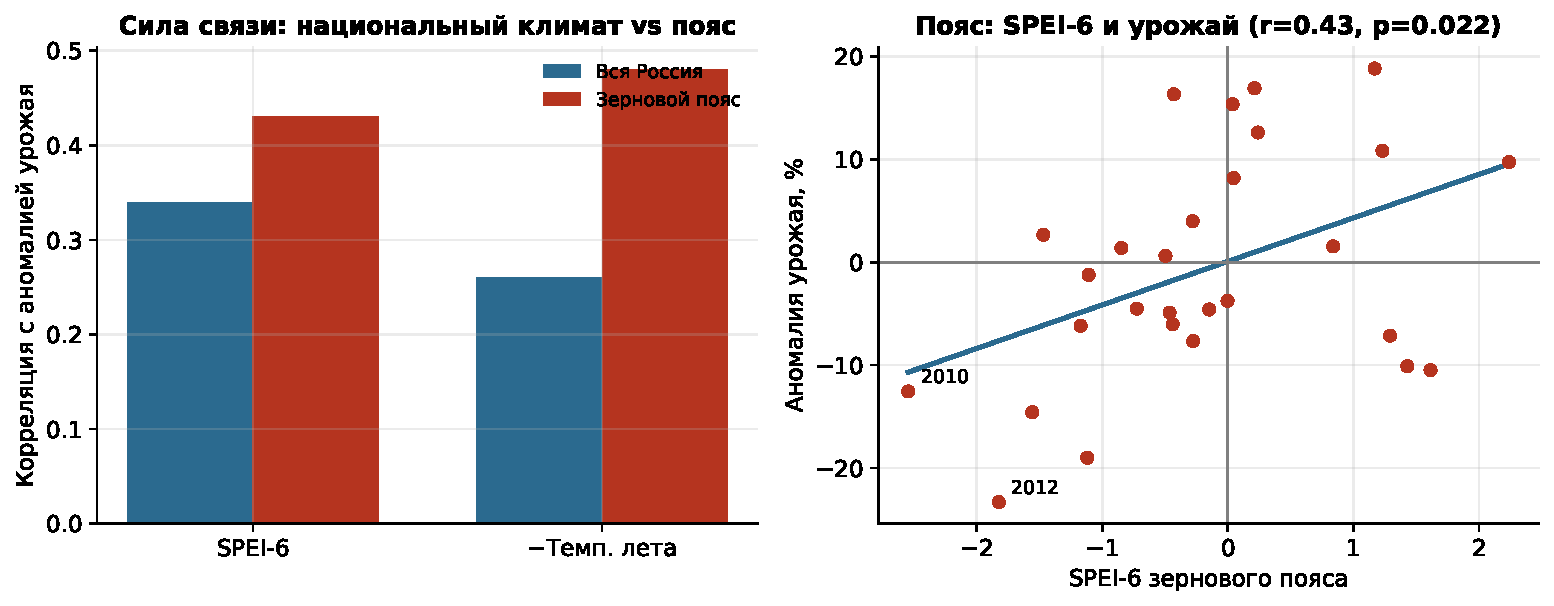
\includegraphics[width=\textwidth]{fig09_belt_vs_national.pdf}
\caption{Сила связи «засуха–урожай»: климат всей России против зернового пояса, 1992--2019. Источник: расчёты авторов по данным GPCC~\cite{gpcc2013}, GHCN-CAMS~\cite{ghcncams2008}, FAOSTAT~\cite{faostat2026}}
\label{fig:belt}
\end{figure}

\subsection{Ограничения}

Пространственное усреднение климата частично преодолено переходом к климату зернового пояса (подраздел выше); урожайность, однако, по-прежнему взята на национальном уровне FAOSTAT, и полное снятие ограничения требует субнациональных данных урожайности (Росстат). Технологический тренд оценён эмпирически. Эти ограничения определяют направления усложнения (раздел~2.3). Робастность выводов проверена: результаты устойчивы к способу детрендирования (аномалии по LOESS и по локальной полиномиальной аппроксимации с исключением оцениваемого года коррелируют на уровне $0{,}98$), а денежные оценки устойчивы к выбору контрфакта и системы цен.

% =====================================================================
%  ЗАКЛЮЧЕНИЕ
% =====================================================================
\structhead{Заключение}

В работе на реальных открытых данных количественно оценено влияние засух на урожайность зерновых и связанные с ним экономические потери. Выполнен обзор литературы (более~20 научных работ), сформирован воспроизводимый набор данных и рассчитаны индексы засушливости SPI и SPEI с собственной программной реализацией. Установлено, что засушливость значимо связана с аномалиями урожайности: в панели с фиксированными эффектами коэффициент корреляции для SPEI-6 составляет $0{,}42$ ($p<0{,}001$), а повышение SPEI на одно стандартное отклонение соответствует приросту урожайности пшеницы на $4$--$6\,\%$; экстремальная жара лета снижает урожай примерно на $7\,\%$ на стандартное отклонение. Модели машинного обучения (CatBoost, случайный лес) при стандартной кросс-валидации объясняют около $37\,\%$ дисперсии аномалий урожая, превосходя линейные методы; при строгой проверке на новых годах качество падает до $\approx7\,\%$, что указывает на ограниченную предсказуемость и преимущественно неклиматический характер бо́льшей части изменчивости. Прямые потери сбора зерновых в России в засушливые годы оценены в $1$--$3$~млрд долл. США (до $18\,\%$ ожидаемой стоимости продукции), а накопленно за 2000--2022~гг. составляют порядка $6{,}5$--$11$~млрд долл. в зависимости от метода. Переход от усреднённого по стране климата к климату зернового пояса усиливает связь засушливости с урожаем (корреляция с летней жарой возрастает с $0{,}26$ до $0{,}48$), что подтверждает главный вывод: основной резерв точности заключён в пространственном разрешении данных.

Поставленные задачи выполнены. Намечен план усложнения постановки: переход на субнациональный уровень, учёт фенологии и данных дистанционного зондирования, имитационное моделирование роста культур и климатические сценарии. Весь программный код и данные опубликованы в репозитории (приложение~А).

% =====================================================================
%  СПИСОК ИСТОЧНИКОВ
% =====================================================================
\clearpage
\printbibliography[heading=bibintoc,title={Список использованных источников}]

% =====================================================================
%  ПРИЛОЖЕНИЕ
% =====================================================================
\appendix
\section*{Приложение А. Программный код и структура репозитория}
\addcontentsline{toc}{section}{Приложение А. Программный код и структура репозитория}

Исходный код, данные и инструкции по запуску опубликованы в репозитории GitHub:\\
\texttt{https://github.com/moura27272727-pixel/agro-drought-losses}\\[4pt]
Структура: \texttt{src/}: модули анализа (расчёт SPI/SPEI, сборка панели, корреляции, панельные регрессии, ML, оценка убытков); \texttt{data/}: исходные и обработанные данные с описанием источников; \texttt{figures/}: графики; \texttt{report/}: настоящая работа; \texttt{slides/}: презентация. Полный прогон: командой \texttt{python src/run\_all.py}.

\end{document}
